% Asset ID: A21TrigonometricFunctionsTikZ-001
% Source: Chapter 6 Trigonometric Functions PDF/transcript + CCEA A21-TRIG-LO004
% Related lesson section: Core Theory - New reciprocal Pythagorean identities
% Purpose: Derive reciprocal Pythagorean identities from sin^2(theta)+cos^2(theta)=1.

\documentclass[tikz,border=8pt]{standalone}
\usepackage{amsmath}
\usetikzlibrary{arrows.meta, positioning}
\begin{document}
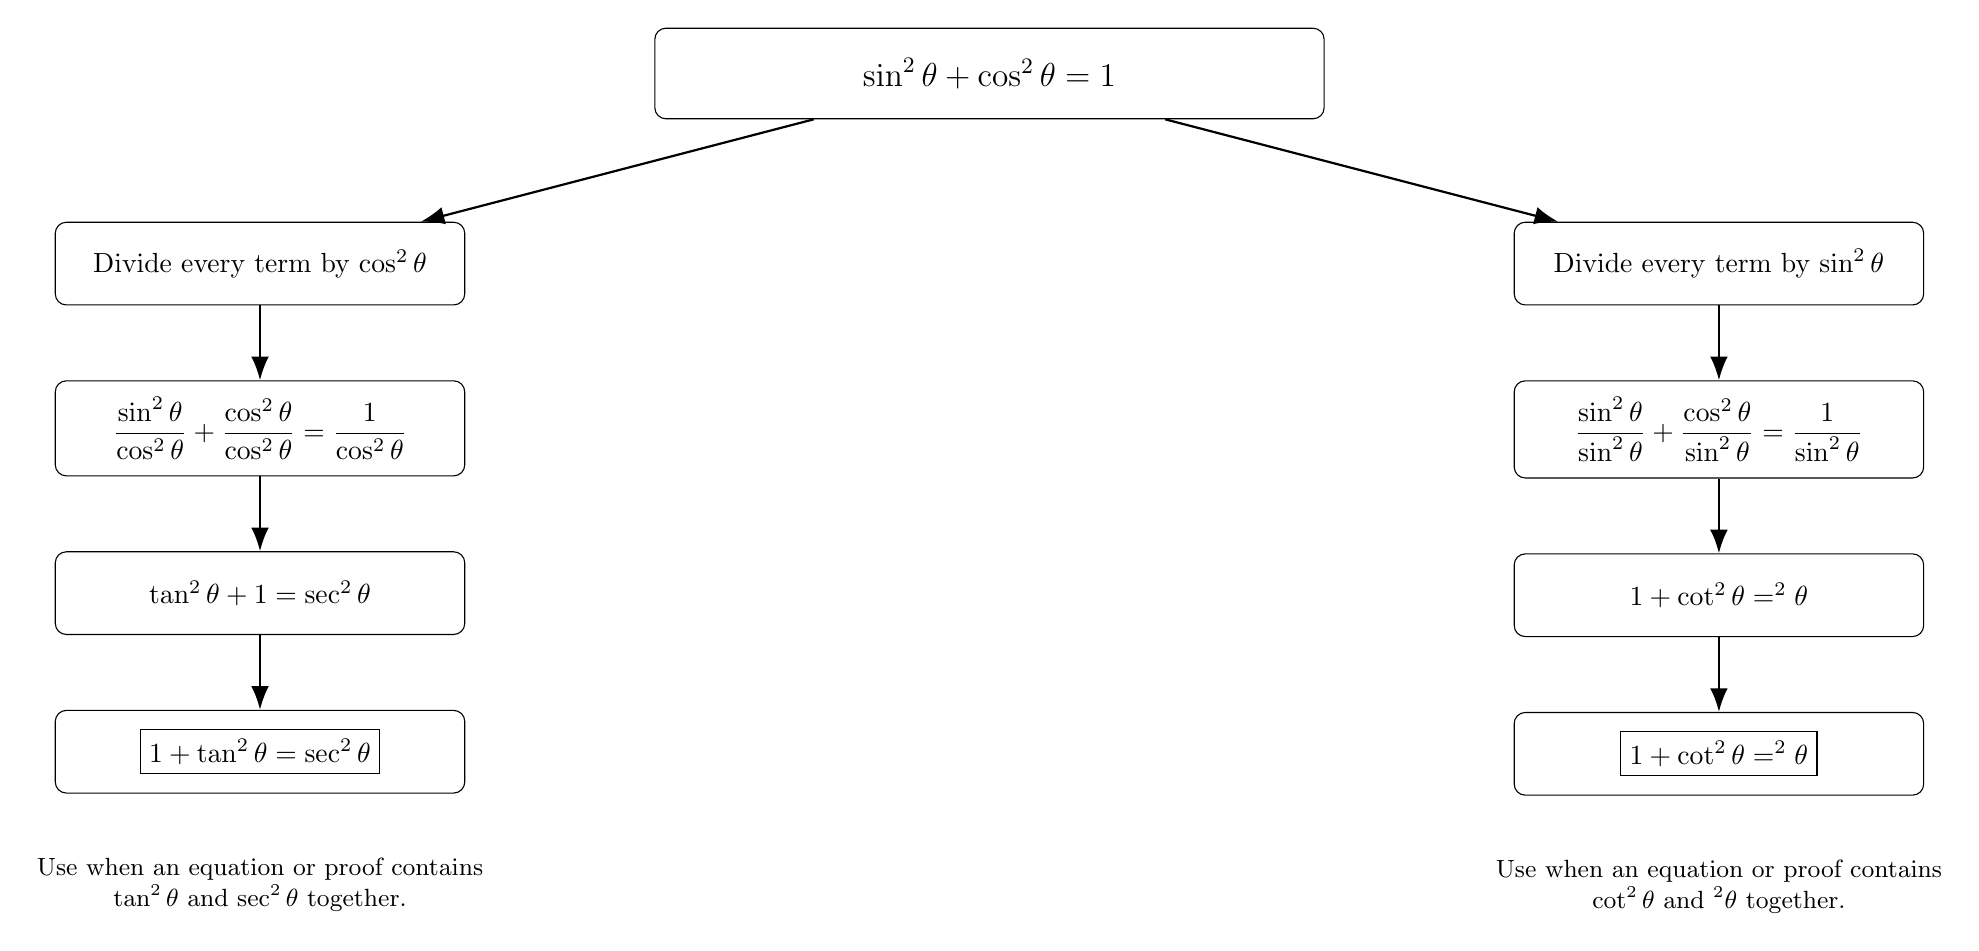
\begin{tikzpicture}[box/.style={draw,rounded corners,align=center,minimum width=5.2cm,minimum height=1.05cm,inner sep=6pt},titlebox/.style={draw,rounded corners,align=center,minimum width=8.5cm,minimum height=1.15cm,inner sep=7pt,font=\large\bfseries},arrow/.style={-{Latex[length=3mm]},thick},note/.style={align=center,font=\small}]
\node[titlebox] (start) at (0,0) {$\sin^2\theta+\cos^2\theta=1$};
\node[box, below left=1.3cm and 2.4cm of start] (dividecos){Divide every term by $\cos^2\theta$};
\node[box, below=0.95cm of dividecos] (cosstep){$\dfrac{\sin^2\theta}{\cos^2\theta}+\dfrac{\cos^2\theta}{\cos^2\theta}=\dfrac{1}{\cos^2\theta}$};
\node[box, below=0.95cm of cosstep] (tansec){$\tan^2\theta+1=\sec^2\theta$};
\node[box, below=0.95cm of tansec] (identityone){$\boxed{1+\tan^2\theta=\sec^2\theta}$};
\node[box, below right=1.3cm and 2.4cm of start] (dividesin){Divide every term by $\sin^2\theta$};
\node[box, below=0.95cm of dividesin] (sinstep){$\dfrac{\sin^2\theta}{\sin^2\theta}+\dfrac{\cos^2\theta}{\sin^2\theta}=\dfrac{1}{\sin^2\theta}$};
\node[box, below=0.95cm of sinstep] (cotcosec){$1+\cot^2\theta=\cosec^2\theta$};
\node[box, below=0.95cm of cotcosec] (identitytwo){$\boxed{1+\cot^2\theta=\cosec^2\theta}$};
\draw[arrow] (start) -- (dividecos);\draw[arrow] (dividecos) -- (cosstep);\draw[arrow] (cosstep) -- (tansec);\draw[arrow] (tansec) -- (identityone);
\draw[arrow] (start) -- (dividesin);\draw[arrow] (dividesin) -- (sinstep);\draw[arrow] (sinstep) -- (cotcosec);\draw[arrow] (cotcosec) -- (identitytwo);
\node[note, below=0.7cm of identityone] {Use when an equation or proof contains\\$\tan^2\theta$ and $\sec^2\theta$ together.};
\node[note, below=0.7cm of identitytwo] {Use when an equation or proof contains\\$\cot^2\theta$ and $\cosec^2\theta$ together.};
\end{tikzpicture}
\end{document}
